\chapter{Pilotforsøg}\vspace{-.75cm}
\textit{Dette bilag beskriver pilotforsøget, som er nødvendigt i forhold til testmåling og design af aktivitetsmåleren. Der undersøges tre forskellige placeringer af sensoren i tre forskellige aktivitetsformer på fire forsøgspersoner.}

\section{Teori}
\textbf{Grundlæggende teori eller henvis tilbage bevægelsesanalysen (Hvis der er en)}

\section{Formål}
For at kunne modificere og tilpasse softwaren til CY8CKIT-043 PSoC 4 M-Series Prototyping Kit er det nødvendigt at kende signalets frekvensindhold og vide, hvordan forskellige aktivitetsformer påvirker sensoren. Målingerne skal undersøges for at kunne lave en algoritme, som kan få sensoren til at skelne imellem de pågældende aktivitetsformer. Derudover skal det bestemmes, hvor sensoren skal placeres på kroppen for mest optimalt udbytte. Derfor er formålet med pilotforsøget følgende:
\begin{itemize}
	\item Bestemme hvordan sensoren påvirkes af gang, løb og cykling.
	\item Undersøge hvor mange g-kræfter sensorens målinger ændrer sig alt efter placering på kroppen.
	\item Undersøge bevægelsesmønstret i signalet i forhold til placering af sensor.
	\item Bestemme frekvensindholdet for signalet.
\end{itemize}

\section{Materiale}
\begin{itemize}
	\item Løbebånd med justerbar hastighed og sikkerhedsbæresele.
	\item Motionscykel.
	\item Shimmer3 sensor.
	\item Computer med programmet Multi Shimmer Sync version ?.
\end{itemize}

\section{Fremgangsmåde}
Inden forsøget skal computeren med programmet Multi Shimmer Sync forbindes via Bluetooth med Shimmer3 sensoren. Herefter kalibreres Shimmer3 accelerometeret ved hjælp af kalibreringsklodsen og samplingsfrekvensen indstilles til 500 Hz.\fxnote{Gyroskop trækker for meget, og systemet vil selv sige til, hvis frekvensen er for høj - sættes typisk til 1024 Hz, men derfor sættes den i dette tilfælde kun til 500 Hz} %Alle andre har indstillet til 1024 Hz, men kan ikke sige hvorfor.
Der oprettes en mappe for hver forsøgsperson, som yderligere inddeles i tre mapper efter aktivitetsform. Herunder navngives datafilerne fra målingerne i forhold til placering af sensor, som for eksempel "Forsoegsperson\_1 $\rightarrow$ Gang $\rightarrow$ Ankel".\fxnote{Diskuterres om det er for dybdegående - nogle er for og andre er imod}
Der foretages en testmåling med sensoren, hvor den tændes kortvarigt mens den påvirkes med 1 g. Hvis data fra denne testmåling optages og skildres korrekt er sensoren klar til forsøget.

Forsøget udføres med fire forsøgspersoner. Hver forsøgsperson skal henholdsvis gå, løbe og cykle. Derudover foretages en måling, hvor forsøgspersonen skal nå op til maksspurt fra hvile med konstant stigningsintervaller. Hvor hver af disse fire målinger skal sensoren placeres på tre forskellige steder, som kan ses på \figref{fig:sensor_placering}. Dette giver $4 x 3 = 12$ målinger for hver forsøgsperson og derfor 48 målinger i alt. Derfor er korrekt placering og navngivning af datafilerne yderst essentiel. \\ 
Gang har tre hastigheder - slentre med 2 mph, almindelig gang med 3 mph og frisk gang med 4 mph. Derfor er almindelig gang valgt som tempoet for gangmålingen, hvilket er 3 mph = 4,8 $\sfrac{km}{t}$.\fxnote{Miles per hour omregnes til kilometer i timen ved at gange med 1,61} Løb har ligeledes tre hastigheder - 6, 7 og 8 mph. Derfor er der igen valgt midtværdien på 7mph = 11.3 $\sfrac{km}{t}$ til løbemålingen. Cykling kan have en moderat intensitet på 10-12 mph og en høj intensitet på 12-14 mph. Derfor er midtpunktet valgt, som er 12 mph = 19,3 $\sfrac{km}{t}$. \citep{Miles2007}
%Inden optagelse af data påbegyndes, skal forsøgspersonen have udført den pågældende aktivitet i et minut for at sikre homogen cyklus i den fysiske udførsel. \\
Sensoren skal placeres tre forskellige steder under hvert forsøg på forsøgspersonens højre ben: proximalt over den laterale malleolus, medialt på den ventrale side af tibia og distalt for patella, som illustreret på \figref{fig:sensor_placering}.
\begin{figure}[H]
	\centering
	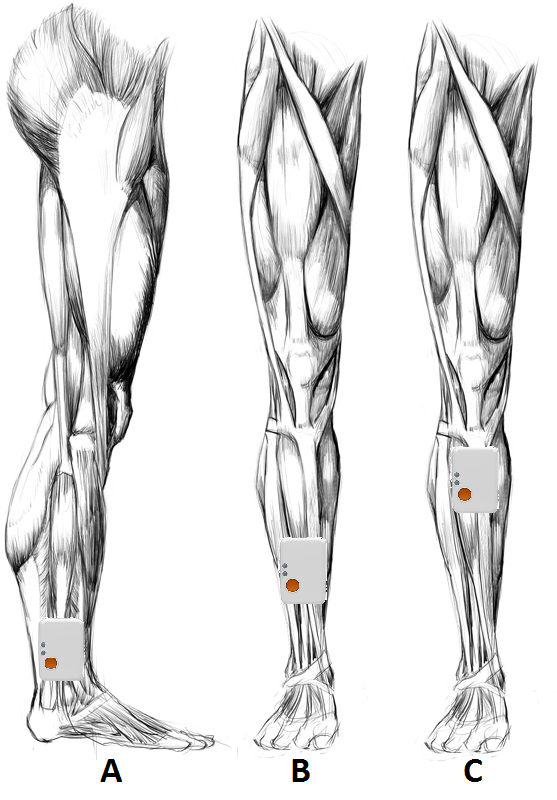
\includegraphics[scale=0.6]{figures/qBilag/Sensor_placering.png}
	\caption{På figuren ses, hvor sensoren skal placeres under pilotforsøget. Placering A viser sensoren siddende proximalt over den laterale malleolus. Placering B illustrerer sensoren, når den er medialt på den ventrale side af tibia. I placering C er sensoren distalt for patella. (Modificeret fra \cite{Perna2016,Shimmer2016})}
	\label{fig:sensor_placering}
\end{figure}
\begin{itemize}
	\item Den første forsøgsperson får fastgjort sensoren i placering A, B eller C - se \figref{fig:sensor_placering}, og gør klar til den pågældende aktivitet ved et stå op kanten af løbebåndet eller sætte sig op på cyklen. Ved aktiviteter på løbebånd skal forsøgspersonen bære sikkerhedsbæresele, som beskytter i tilfælde af fald.
	\begin{itemize}
		\item Ved gang indstilles løbebåndet til 4.8 $\sfrac{km}{t}$ mens forsøgspersonen står på siden af løbebåndet. Optagning af data påbegyndes, mens forsøgspersonen står stille i 0 sekunder for at optage en baseline for sensorens påvirkning. Herefter træder forsøgspersonen op på løbebåndet og får 20 sekunder til at opnå homogen cyklus i den fysiske udførsel. Efter disse to sekunder optages der yderligere et minut, hvorefter dataoptagelsen stoppes.
		\item Ved løb indstilles løbebåndet til en acceptabel fart, hvor forsøgspersonen kan hoppe på uden fare. Der optages 10 sekunders baseline af sensorens påvirkning, mens forsøgspersonen står på kantet af løbebåndet og udfører ikke noget aktivitet. Herefter hopper forsøgspersonen på løbebåndet og får 20 sekunder til at opnå homogen cyklus i den fysiske udførsel. Derudover skrues løbebåndets hastighed op til 11.3 $\sfrac{km}{t}$ inden for disse 20 sekunder. Målingen fortsættes i endnu et minut inden forsøget afsluttes.
		\item Ved stigning i intensitet skal forsøgspersonen stå stille på løbebåndet mens optagningen påbegyndes og der optages en 10 sekunders baseline. Herefter skal løbebåndets hastighed stige fast med et konstant interval, indtil maksspurt er opnået. Dette er en subjektiv vurdering, hvorfor den konstante stigning i hastighed er essentiel og skal noteres i forhold til tid.
		\item Ved cykling skal forsøgspersonen sidde på cyklen og have pedalerne placeret i samme højde. Der optages en 10 sekunders baseline, hvorefter forsøgspersonen hurtigst muligt og uden at skifte gear skal komme op på 20.9 $\sfrac{km}{t}$. Når dette er opnået, optages signalet i yderligere et minut.
	\end{itemize}
	\item Efter hver måling skal forsøgspersonen restituere i 10 minutter for at sikre, at der ikke sker en kompensering i gang- eller løbecyklus på grund af træthed. %Der tages dog ikke højde for muskeltræthed, da det vurderes, at fysisk aktivitet af denne form ikke vil lede til muskeltræthed inden for disse korte intervaller.\fxnote{Skal vi have en kilde på det her?}
	\item Den pågældende fysiske aktivitet gentages tre gange for hver forsøgsperson, da sensoren skal placeres anderledes for hver gang. Sensoren Shimmer3 skal kalibreres for hvert placeringsskifte.
\end{itemize}

\section{Databehandling}

\section{Resultater}

\section{Diskussion}

\section{Konklusion}

%% Opgaver - rettelser
% Man skal markere på forsøgspersonen med tush eller andet hvor sensoren skal placeres